\begin{frame}
\frametitle{Søgning med eksempelbilleder}
\begin{figure}[H]
	\centering
	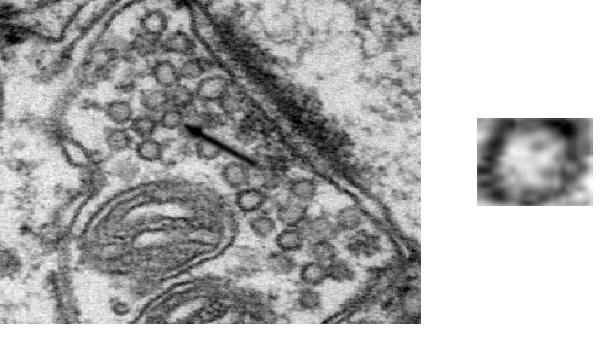
\includegraphics[scale=0.4]{img/finalmethod/cell2.png}
\end{figure}
\end{frame}

\begin{frame}
\frametitle{Foldning med eksempelbilleder}
\begin{figure}[H]
	\centering
	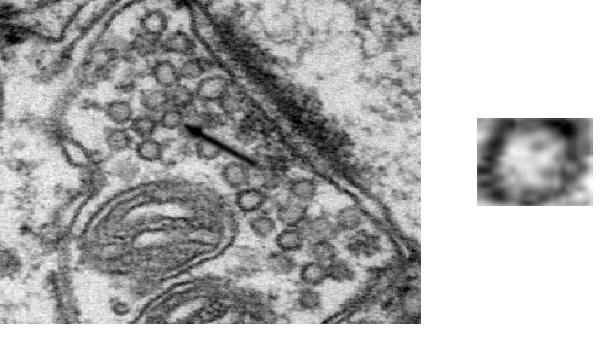
\includegraphics[scale=0.4]{img/finalmethod/cell2.png}
\end{figure}
\begin{figure}[H]
	\centering
	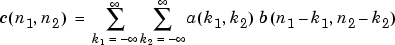
\includegraphics[scale=0.6]{img/finalmethod/math_c5.png}
\end{figure}
\end{frame}

\begin{frame}
\frametitle{Foldning med eksempelbilleder}
\begin{figure}[H]
	\centering
	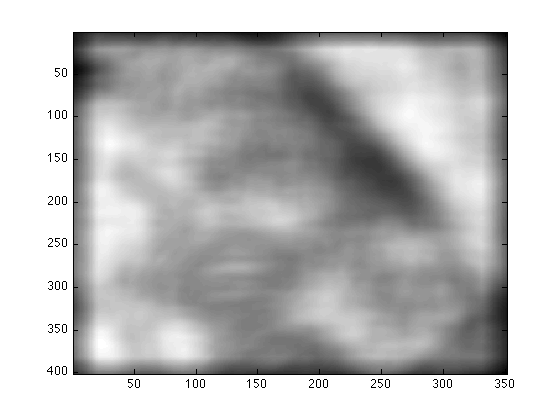
\includegraphics[scale=0.6]{img/finalmethod/convolve.png}
\end{figure}
\end{frame}

\begin{frame}
\frametitle{Afstand til eksempelbilleder}
\begin{align*}
	||\vec{I}-\vec{J}||^2 = (\vec{I}-\vec{J})^T(\vec{I}-\vec{J}) = \vec{I}^T\vec{I} + \vec{J}^T\vec{J}-2\vec{I}^T\vec{J}
\end{align*}
\end{frame}

\begin{frame}
\frametitle{Afstand til eksempelbilleder}
\begin{align*}
	||\vec{I}-\vec{J}||^2 = (\vec{I}-\vec{J})^T(\vec{I}-\vec{J}) = \vec{I}^T\vec{I} + \vec{J}^T\vec{J}-2\vec{I}^T\vec{J}
\end{align*}

\begin{align*}
	\sum_m\sum_n \left(\frac{I_{ij}-mean(I_{ij})}{std(I_{ij})}-\frac{J-mean(J)}{std(J)}\right)^2
\end{align*}
\end{frame}